\chapter*{Chapter 1}
\markboth{Chapter 1 }{Host organization and project context} %pour afficher l'entete
\addcontentsline{toc}{chapter}{I Host organization and project context}

\textsc{\textbf {\Huge Host organization and project context}} \\ 

\setcounter{chapter}{1}
\section{Introduction}
This chapter welcomes the host institution, highlighting its organizational nature and principal research focus areas. It follows by providing the setting for the development of the project, stating the problem identified, and providing the main aim of the work. Finally, the methodology adopted to implement the project is described, as well as the time frame scheduled as evident on the Gantt diagram.

\section{Host organization}
This section presents the host institution of the project. It provides an overview of Chemnitz University of Technology, describes the structure of the Measurement and Sensor Technology (MST) laboratory, and highlights the role of German cooperation programs in supporting the project.
\subsection{Overview of the university}
Chemnitz University of Technology is a prestigious public German university founded in
1836 in Chemnitz, Saxony and was promoted to a university of technology, in 1963. With
approximately 1,500 science, engineering and management staff members, and 9000 students,
Chemnitz University of Technology is the third largest Saxony university.\cite{TUChemnitz}
The official organization logo is shown in the following figure 1.1.
\begin{figure}[H]
    \centering
    
\includegraphics[width=0.4\linewidth]{imagess/TU_Chemnitz_Logo_gruen_RGB-2048x1341 (1).png}
    \caption{Technische Universitat Chemnitz.\cite{TUChemnitz}}
    \label{fig:enter-label}
\end{figure}

The internship was held at the Faculty of Electrical Engineering and Information Technology, which is composed of multiple institutes. Different professorships that address different subtopics under the broad umbrella of the faculty are housed in each institute. The project was done under the leadership of the Measurement and Sensors Technology (MST) professorship.
The MST professorship's official logo is illustrated in figure I.3.\\
\begin{figure}[H]
    \centering
    
\includegraphics[width=0.2\linewidth]{imagess/MST_logo (1).png}
    \caption{Measurement and Sensors Technology department.\cite{TUChemnitzMUST}}
    \label{fig:enter-label}
\end{figure}



\subsection{Laboratory structure and organization}
The Measurement and Sensor Technology (MST) laboratory conducts multidisciplinary research in the development of next-generation sensor systems and measurement methods. Its main fields of research are\cite{TUChemnitzMUST}:
\begin{itemize}
\item \textbf{Impedance spectroscopy}\\
Investigation of electrical impedance behavior to analyze material properties and processes, with biomedical diagnostics, material science, and process control purposes.
\item \textbf{Wireless sensors}\\
Development of sensor systems with wireless communication capabilities for real-time data acquisition, remote monitoring, and IoT network integration.

\item \textbf{Nanocomposite sensors}\\
Designing sensors based on composite and nanostructured materials to enhance sensitivity, selectivity, and functional performance.

\item \textbf{Electrochemical sensors}\\
Exploring electrochemical mechanism-based sensors for the detection of chemical and biological compounds, enabling applications in healthcare, environmental monitoring, and industrial processes.

\item \textbf{Smart wearables}\\
Creating wearable sensor systems that combine advanced sensing, signal processing, and wireless communications to enable health monitoring and activity tracking.
\end{itemize}
\subsection{German cooperation}
The German Academic Exchange Service or better knows as Deutscher Akademischer Aus-
tauschdienst (DAAD) is the world’s largest funding organisation for the international exchange of students and researchers. Originating from a student initiative in 1925, the DAAD has developed into a registered association of German universities and student bodies.This project was funded by the DAAD as part of its commitment to fostering international scientific collaboration. 
\cite{DAAD}\\
The official logo of the German Academic Exchange Service is shown in figure I.3
\begin{figure}[H]
    \centering
    
\includegraphics[width=0.4\linewidth]{imagess/DAAD-Logo.jpg}
    \caption{The German Academic Exchange Service.\cite{DAAD}}
    \label{fig:enter-label}
\end{figure}

\section{Project context} 
Biomedical engineering has come to embrace increasingly non-invasive imaging modalities to provide real-time observation of physiology without the risks of ionizing radiation or invasive procedure. Of the modalities, Electrical Impedance Tomography (EIT) stands out in terms of cost-effectiveness, portability, and the capacity to retrieve functional information regarding tissues. By injecting small alternating currents into the body and measuring the voltage patterns produced, EIT reconstructs conductivity or impedance distributions, enabling applications for pulmonary function monitoring, muscle activity measurement, and tissue characterization.

The past decade has witnessed the evolution of EIT research from one-frequency static systems to multi-frequency approaches based on the realization that biological tissues have frequency-dependent electrical properties. Multi-frequency measurements can identify both structure and biochemical information and provide higher diagnostic sensitivity. In most existing systems, however, such frequencies are measured in sequence, which limits temporal resolution and renders them less effective in coping with the fast physiological processes like respiration cycles, muscle activations, or rapid gestures.

Simultaneous multi-frequency EIT (SMF-EIT) offers a promising option by enabling simultaneous injection of more than one sinusoidal current at various frequencies and corresponding voltage responses to be obtained in real-time. This method has the potential to provide spectral information without losing temporal content, allowing for enhanced and dynamic biomedical imaging. Yet, it is hard to use SMF-EIT in hardware design, frequency separation, signal processing, and computational efficiency when focusing on embedded or wearable platforms where size, power consumption, and processing speed are of top priority.

In this context, the project was started in the Measurement and Sensor Technology (MST) Laboratory of Chemnitz University of Technology. Operation focuses on the design and development of an embedded SMF-EIT measurement system capable of generating, capturing, and processing multi-frequency signals. Design development is focused on moving from laboratory-oriented EIT systems to portable application-specific biomedical devices, which will be advantageous for rehabilitation monitoring, lung function analysis, and human–machine interfaces under gesture control.
\section{Problematic}
Electrical Impedance Tomography (EIT) has gained increasing attention as a safe, low-cost, and portable non-invasive imaging modality due to its ability to deliver diagnostic information regarding physiological properties of the tissue. It administers small alternating currents through electrodes placed on the body surface and measures the voltage responses to image the internal tissue impedance distribution. Impedance is physiologically sensitive to properties like muscle contraction, blood flow, and tissue composition.

While promising, conventional EIT systems are plagued by a series of shortcomings that degrade their real-time performance and diagnostic capability. One of the major shortcomings is the way they treat frequencies: most systems handle a single frequency or perform sequential sweeps of frequencies, which is time-consuming and not adequate for the observation of dynamic, frequency-dependent tissue behavior. In medical applications, tissues exhibit different impedance characteristics at different frequencies. Hence, it is essential to get this spectral information in real-time for enhancing the spatial and functional resolution of EIT devices.

\section{Project objectives}
This project aims to develop an embedded Simultaneous Multi-frequency Electrical Impedance Tomography (SMF-EIT) system that overcomes the limitations of traditional EIT setups. The specific objectives are:
\begin{itemize}
 
\item \textbf{Design and implementation of the acquisition System}\\
Develop a compact, efficient hardware platform based on the STM32G474 micro-controller, leveraging its high-speed ADCs for real-time multi-channel sampling of voltage and current signals.
\item \textbf{Simultaneous current injection and voltage Measurement}\\
Inject a multi-frequency excitation signal into the system and accurately measure the resulting current and boundary voltages at the boundary electrodes .

\item \textbf{Data acquisition and signal processing}\\
Acquire raw ADC samples from the micro-
controller and transmit them to a host computer for offline processing(
frequency component extraction, magnitude and phase calculation, and
impedance estimation).

\item \textbf{Impedance computation and data formatting}\\
From the processed voltage and current signals, compute the complex impedance between electrode pairs at each frequency. Format the results for potential use in classification algorithms or image reconstruction pipelines.

\item \textbf{Experimental validation on a test-tank experiments}\\
Evaluate the system’s performance using a controlled experimental setup (a water tank with electrodes) to verify measurement accuracy, phase stability, and frequency separation capability.



\end{itemize}

\section{Work methodology and gantt diagram}
The project was followed by a well-planned methodology for efficient progress and systematized confirmation of results. The work was divided into clearly defined phases, with literature review to establish the theoretical foundation, system design, hardware development, and firmware implementation. Experimental confirmation was carried out through the utilization of a test-tank modal, in which data acquisition and analysis were performed in parallel to optimize the process. The final phase involved documentation and report. The
elaborate timeline, as represented in the Gantt diagram 1.4, indicates the planned duration,
order, and overlap of the tasks to facilitate a rational flow from idea to final validation.

\begin{figure}[H]
    \centering
    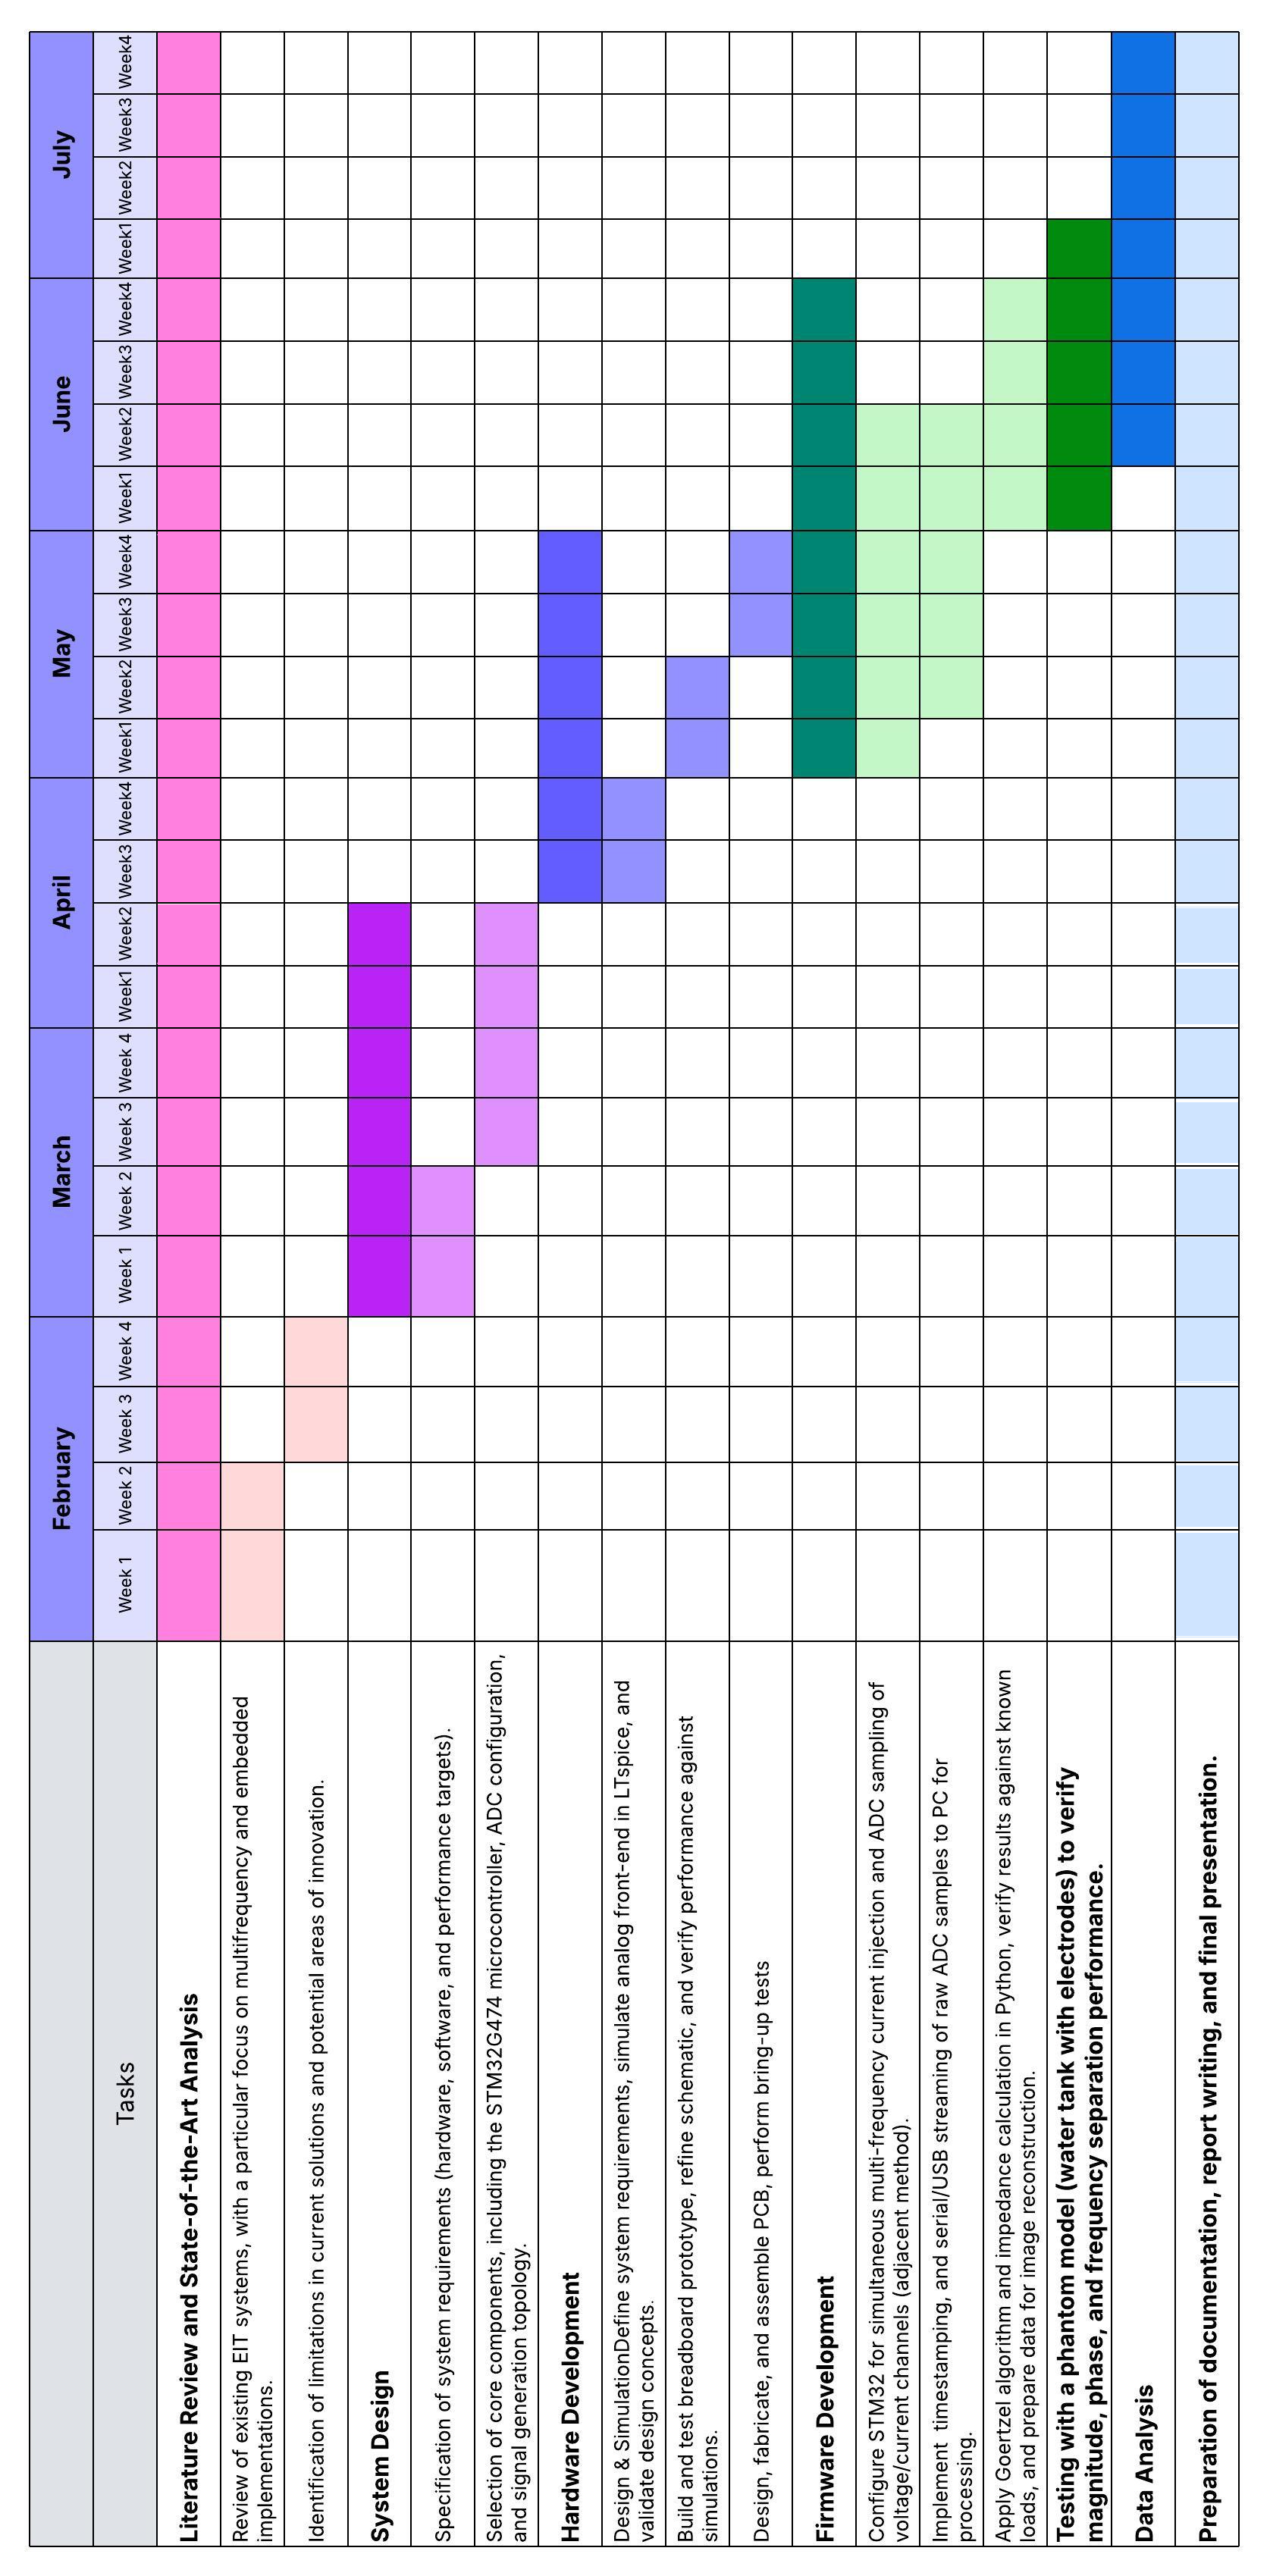
\includegraphics[width=0.7\textwidth]{imagess/gantt.png}
    \caption{Project work methodology and timeline (Gantt chart).}
    \label{fig:stability_lowfreq}
\end{figure}

\section{ Conclusion}
This chapter provided an overview of the host organization, structure, facilities, and international
associations to place the professional environment within which
the project was conducted. It also explained the background and motivation behind the work,
defined the problem statement, and set the project objectives. Finally, the adopted work
methodology and corresponding Gantt diagram were provided to display the formalized
procedure and scheduled plan for project completion. This forms the foundation of subsequent
chapters, which will record the technical design, development, and verification of the proposed
simultaneous multi-frequency Electrical Impedance
Tomography (EIT) system for biomedical purposes.
